% paper.tex
% ACM sigmetric format
% Author: L. K. Melhus and R. E. Jensen
%\documentclass{acm_proc_article-sp}
\documentclass[10pt, conference, compsocconf]{IEEEtran}
\usepackage{graphicx}
\usepackage{pgfplots}
\usepackage{pgfplotstable}
\usepackage{filecontents}
\usepackage{tikz}
\usepackage{listings}
\usepackage{mathtools}
\usepackage{underscore}
\usepackage{url}
\usepackage{lmodern} % Much clearer text
\usepackage[utf8]{inputenc}
\usepackage{hyperref} % For PDF metadata
%\usepackage{enumitem} % Controlling list styling
%\usepackage[font=small,skip=0pt]{caption}
%http://tex.stackexchange.com/questions/94016/how-to-reduce-space-between-image-and-its-caption
\usepackage[font=small,belowskip=-10pt,aboveskip=0pt]{caption}

%\setlength{\intextsep}{10pt plus 2pt minus 2pt}

%\setlength{\belowcaptionskip}{-5pt}
% too much?

%\captionsetup[table]{aboveskip=-25pt}

%\setlength{\dblfloatsep}{-15pt}

%\addtolength{\belowcaptionskip}{15pt}

\usetikzlibrary{patterns,shapes,positioning,calc}

\lstset{language=C, basicstyle=\ttfamily, columns=flexible, belowskip=0pt}

%\setlist{topsep=0pt}

\pgfplotsset{compat=1.8}

\newcommand{\perfctr}[1] {
  {\lowercase{#1}}
}

\begin{document}

\hypersetup
{
%    pdfauthor={L. K. Melhus and R. E. Jensen},
    pdfauthor={Anonymous and Anonymous},
    pdfsubject={Identification of an underlying mechanism that causes measurement bias},
    pdftitle={Measurement Bias from Address Aliasing},
    pdfkeywords={4K address aliasing, BLAS, heap allocators, measurement bias, memory disambiguation, performance counters}
}

%\conferenceinfo{SIGMETRICS}{2015 Portland, Oregon USA}
%\CopyrightYear{2015}
%\acmVolume{V}
%\acmNumber{N}
%\acmArticle{A}
%\acmYear{YYYY}
%\acmMonth{0}

% Page headers
%\markboth{L. K. Melhus and R. E. Jensen}{Measurement Bias from Address Aliasing}

\title{Measurement Bias from Address Aliasing}

%\numberofauthors{2}
 
\iffalse
% names here
\author{
% You can go ahead and credit any number of authors here,
% e.g. one 'row of three' or two rows (consisting of one row of three
% and a second row of one, two or three).
%
% The command \alignauthor (no curly braces needed) should
% precede each author name, affiliation/snail-mail address and
% e-mail address. Additionally, tag each line of
% affiliation/address with \affaddr, and tag the
% e-mail address with \email.
%
% 1st. author

\alignauthor
Lars Kirkholt Melhus\\
       \affaddr{Norwegian University of Science and Technology}\\
       \affaddr{Sem Sælands vei 9}\\
       \affaddr{7491 Trondheim, Norway}\\
       \email{lars.kirkholt.melhus@gmail.com}
% 2nd. author
\alignauthor
Rune Erlend Jensen\\
       \affaddr{Norwegian University of Science and Technology}\\
       \affaddr{Sem Sælands vei 9}\\
       \affaddr{7491 Trondheim, Norway}\\
       \email{runeerle@idi.ntnu.no}

\alignauthor
Anonymous\\
       \affaddr{Anonymous University}\\
       \affaddr{Anonymous}\\
       \affaddr{Anonymous, Anonymous}\\
       \email{anonymous@anonymous.com}
% 2nd. author
\alignauthor
Anonymous\\
       \affaddr{Anonymous University }\\
       \affaddr{Anonymous}\\
       \affaddr{Anonymous, Anonymous}\\
       \email{anonymous@anonymous.com}
}
\fi

\author{\IEEEauthorblockN{Authors Name/s per 1st Affiliation (Author)}
\IEEEauthorblockA{line 1 (of Affiliation): dept. name of organization\\
line 2: name of organization, acronyms acceptable\\
line 3: City, Country\\
line 4: Email: name@xyz.com}
\and
\IEEEauthorblockN{Authors Name/s per 2nd Affiliation (Author)}
\IEEEauthorblockA{line 1 (of Affiliation): dept. name of organization\\
line 2: name of organization, acronyms acceptable\\
line 3: City, Country\\
line 4: Email: name@xyz.com}
}


\date{19 November 2014}

\maketitle

% Motivation -- Problem statement -- Approach -- Results -- Conclusions
\begin{abstract} % Should be 150 -- 200 words max
Understanding program behavior and obtaining accurate measurements is important in performance analysis.
However, recent research has shown that performance measurements can be \emph{biased} by external factors in unpredictable ways.
Seemingly irrelevant properties---such as the length of your user name---can impact program performance.
In this paper, we identify an important underlying mechanism that causes this type of measurement bias on modern Intel microarchitectures.
Our approach is to use a large set of hardware performance counter measurements to reveal the inner workings of the CPU, and search for correlations over a series of execution contexts.
We find that \emph{address aliasing} can explain bias from two external factors; size of environment variables, and characteristics of dynamically linked heap allocators.

This result not only makes accounting for and avoiding measurement bias much simpler, but also enables explicit optimizations for it.
We demonstrate this by implementing runtime detection and correction of aliasing conditions.
For heap allocators, we show that common implementations tend to give worst case alignment by default, favoring page alignment for large allocations.
The performance impact of unfavorable memory layouts can be significant, with as much as $2x$ speedup in one of our examples.
Finally, we show that even highly optimized BLAS libraries can be impacted by address aliasing.
Our results can enable new architecture specific optimization strategies to account for this phenomenon.
\end{abstract}

% Choose from classification tree http://www.acm.org/about/class/ccs98-html
%\category{C.4}{Performance of Systems}{Measurement techniques; Performance attributes}
%\category{D.3.4}{Processors}{Optimization; Run-time environments}

% Terms come from a fixed list of predefined terms
%\terms{Measurement, Performance}
% Free to choose keywords, but must be in alphabetical order
\begin{IEEEkeywords}
4K address aliasing, BLAS, heap allocators, measurement bias, memory disambiguation, performance counters
\end{IEEEkeywords}

% Minimum is author, year and title
%\acmformat{Lars K. Melhus and Rune E. Jensen. 2014. Measurement Bias from Address Aliasing}




% Acknowledgement of support, author(s) address(es)
%\begin{bottomstuff}
%New Paper, Not an Extension of a Conference Paper.
%Authors' addresses: Lars Kirkholt Melhus, Rune Erlend Jensen, Computer and Information Science Department, Norwegian University of Science and Technology, 
%Sem S{\ae}lands vei 9, Gl{\o}shaugen, 7491 Trondheim, Norway; email: larskirk@alumni.ntnu.no, runeerle@idi.ntnu.no
%\end{bottomstuff}



\section{Introduction}
Accurately measuring the performance of computer programs is important in order to evaluate new algorithms, or compare different implementations.
A key challenge for performance analysts and systems researchers is handling \emph{measurement bias}.
Changes to external factors of the system, such as link ordering or the contents of environment variables, has been shown to have potentially significant impacts on performance in real applications~\cite{Mytkowicz:2009:WrongData}.
The underlying explanation is likely that this changes memory addresses of code or data, which in turn interacts with various low level hardware buffers at runtime.
Because of the complexity of modern processors, it is often hard or even impossible to predict exactly how changes to for example system environment variables ultimately affect program execution.

%\pgfplotstableread{bin/microkernel-cycles-core2.dat}{\microkernelcoretwotable}
\pgfplotstableread{bin/microkernel-core.dat}{\tblmicrokernelcore}
\begin{figure}[t]
  \begin{tikzpicture}
    \begin{axis}[
        title = Core,
        width = \textwidth/2.1,
        height = 4.5cm,
        font = \footnotesize,
        xlabel=Bytes added to environment,
        ylabel=Cycles,
        domain = 0:4096,
        xtick = {0,1024,...,4096},
        xmin = 0,
        xmax = 4096,
        cycle list name = exotic
      ]
      \addplot[ycomb] table[x expr = \thisrowno{0}*16, y = cycles:u] \tblmicrokernelcore ;
    \end{axis}
  \end{tikzpicture}
  \caption{\label{fig:motivation}Performance counter data running the micro-kernel from Figure~\ref{fig:microkernel} under different environment sizes. Notice the clear spike at around 3200 bytes, where the number of cycles executed nearly doubles. Measuring performance in this configuration would give a biased result.}
\end{figure}

\begin{figure}[t]
  \begin{lstlisting}[frame=single, xleftmargin=.01\textwidth, xrightmargin=.01\textwidth]
static int i, j, k;
int main() {
    int g = 0, inc = 1;
    for (; g < 65536; g++) {
        i += inc;
        j += inc;
        k += inc;
    }
    return 0;
}
  \end{lstlisting}
  \caption{\label{fig:microkernel}Microkernel first presented by Mytkowicz et al.\cite{Mytkowicz:2009:WrongData}, showing bias to environment size.}
\end{figure}



A literature study of 88 papers by Mytkowicz et al. showed that the median reported speedup was within the margin of bias, possibly invalidating the claimed speedups~\cite{Mytkowicz:2008:OE&MB}.
To alleviate the impact of measurement bias in performance analysis, researchers have proposed techniques like causal analysis, and randomization of execution contexts~\cite{Mytkowicz:2008:OE&MB}.
Others treat the interaction complexity as a potential optimization problem, using search over variant spaces to find optimal environments~\cite{Knights:2009:BlindOpt}.
Our approach is to analyze isolated programs in detail using hardware performance counters, in an attempt to identify which underlying mechanisms are causing bias.

In Figure~\ref{fig:motivation}, we have reproduced a result originally presented in a paper by Mytkowicz et al.\cite{Mytkowicz:2009:WrongData}, showing how the number of cycles executed for a simple program (Figure~\ref{fig:microkernel}) depends on environment variables.
This example provides the basis for our analysis.
We show how some instances of measurement bias, such as the above, can be explained by \emph{address aliasing}, an artifact of a presumably Intel specific optimization on the out-of-order execution pipeline.
The CPU uses a heuristic for determining whether loads are dependent on previous stores, comparing only the 12 least significant virtual address bits.
Aliased memory accesses can produce false dependencies, and incur performance penalties.
We look at how address aliasing can trigger bias from two external factors; size of system environment variables and configuration of dynamic heap allocation libraries.

Our results show that the cost of aliasing can be significant, exemplified by a simple program with up to $2x$ speedup based in heap address alignment alone.
We also find that many heap allocation libraries tend to produce worst case behavior by default with respect to aliasing, by favoring page alignment for large allocations.
With an understanding of how false dependencies in the CPU can impact performance, measurement bias caused by it can to some extent be predicted and even accounted for in software.
We show how techniques like manual padding of allocations and dynamic detection of aliasing conditions can be used to improve performance. 
Being able to handle address aliasing can give significant speedups, and our findings show potential for further architecture-specific optimizations.

The rest of this paper is structured as follows: Our methodology and experimental setup is explained in the next section.
Then section~\ref{sec:aliasing} introduces ``4K aliasing'', providing necessary background for interpreting the later results.
Section~\ref{sec:environment} presents an analysis of how the size of environment variables causes bias, and in Section~\ref{sec:heap} we go through a similar analysis for bias to heap address alignment.
Finally, in Section~\ref{sec:blas} we look at alias in BLAS libraries.
Related work is discussed in Section~\ref{sec:related}, before we summarize and conclude in Section~\ref{sec:conclusions}.


\section{Experimental Methodology}
\label{sec:methodology}
In order to understand biased behavior it is important to be able to do precise and detailed measurements, without introducing \emph{observer effects}~\cite{Mytkowicz:2008:OE&MB}.
This can be achieved by using performance counters, instrumentation support in hardware that can be used to \emph{count} various events, such as cycles executed, branch misses, instructions fetched, and so on.
Recent Intel architectures have several hundred available events, providing a detailed view of what happens inside the CPU.
Performance counters are supported in the Linux kernel, and can be accessed via a tool called \emph{perf}.
This utility instructs the kernel to enable the processor's Performance Monitoring Unit (PMU), before executing a specified program.
Using this technique avoids modifications to the executed program, unlike tools like PAPI~\cite{PAPI:PortableInterface}.
We use the perf-stat command in all experiments, which accepts raw PMU event codes listed in the reference manual~\cite{Volume3B}.

Reliability of PMU measurements have been evaluated by Weaver and Mckee~\cite{Weaver:2008:PCTrusted}.
The potential issues they find are either handled explicitly or are irrelevant to our setup.
%They find intra-machine variations of up to 1.07\%, 

A small Python script is used to iterate over an exhaustive set of all known counters, which amounts to about 200 on our architecture.
Only a small set of events are collected at a time, to ensure events are actually counted continuously.
We do not use multiplexing between a limited set of counter registers, as it will introduce significant variations~\cite{Wiplove:ImproveEstimation}. % Paper is rename of "Toward Accurate Performance Evaluation using Hardware Counters".
Controlled variations in environment size is performed by setting a dummy environment variable to $n$ number of zero characters, starting from a minimal environment.\footnote{Because perf-stat itself adds a few variables, the environment will never be completely empty.}
Interesting events are identified by computing linear correlation to cycle count, measuring all counters over a series of execution contexts.
% Cache related metrics are monitored in order to rule out cache as the underlying cause of bias, such as hit rates of micro-ops for each level of cache~\cite{OptimizationManual}.
Results are also averaged over multiple runs to reduce potential random error, using built-in perf rerun functionality.

Because bias can be hardware dependent, and to keep the scope of this work manageable, we initially chose to focus our analysis on the 4th generation Intel ``Haswell'' microarchitecture.
We later reproduced similar results for the ``Core'', ``Nehalem'', and ``Ivy Bridge'' microarchitectures as well.
Each setup is described in Table~\ref{tab:machines}, and referenced throughout the paper.

\begin{table}
  \caption{Experimental setups used.\label{tab:machines}}{
  \begin{tabular}{|l|l|}
    \hline
Core          & Intel\textsuperscript{\textregistered{}} Core\texttrademark{}2 Duo P8600 (laptop) \\
              & 64-bit Ubuntu 14.04 LTS (Linux 3.13.0),\\
              & GCC 4.8.2-19ubuntu1 \\ \hline
Nehalem       & Intel\textsuperscript{\textregistered{}} Core\texttrademark{} i7-950 \\
              & 64-bit Ubuntu 12.04 LTS (Linux 3.2.0),\\
              & GCC 4.8.2-19ubuntu1 \\ \hline
% Sandy Bridge  & Intel\textsuperscript{\textregistered{}} Core\texttrademark{} i7-2670QM (laptop) \\
%               & 64-bit Ubuntu 11.04 (Linux 3.0.0) \\ \hline
Ivy Bridge    & Intel\textsuperscript{\textregistered{}} Core\texttrademark{} i5-3470 \\
              & 64-bit Ubuntu 12.04 LTS (Linux 3.8.0),\\
              & GCC 4.8.2-19ubuntu1 \\ \hline
Haswell       & Intel\textsuperscript{\textregistered{}} Core\texttrademark{} i7-4770K \\
              & 64-bit Ubuntu 14.04 LTS (Linux 3.13.0),\\
              & GCC 4.8.2-19ubuntu1 \\ \hline
  \end{tabular}}
\end{table}

Best practices for controlling the execution context were applied, ensuring that we are not affected by any unwanted bias~\cite{Mytkowicz:2009:WrongData}.
Most importantly, this means keeping the memory address space under control.
For security reasons, addresses of the stack, heap and dynamic libraries are often randomized at load time, a technique known as \emph{Address Space Layout Randomization}~\cite{Pax:ASLR,Bhatkar:AddressObfuscation}. 
By disabling ASLR, we are able to execute the same program multiple times with identical virtual address spaces.
All experiments are done on a dedicated machine under minimal load, with \emph{frequency scaling} disabled to keep the CPU's clock speed fixed.
Finally, we disable \emph{Hyper-threading} (HT), which reduces the possibility for resource contention between threads.
Some PMU events also require HT to be turned off, or produce inaccurate results with HT enabled.

% Virtual memory/randomization illustration
\begin{figure}
  \centering
  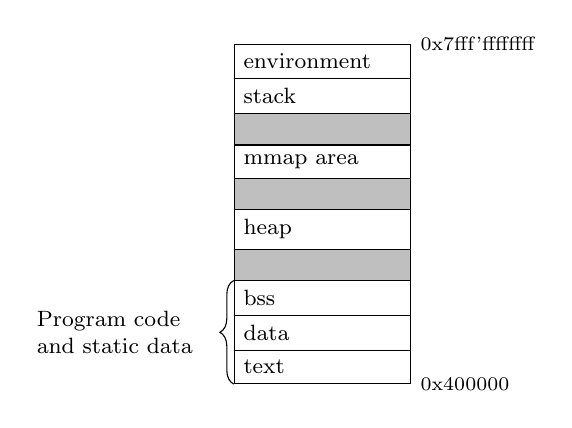
\begin{tikzpicture}[font=\footnotesize]
    % See page 453 in pgf manual
    \node [
      rectangle split, rectangle split parts=10, 
      rectangle split part fill={white, white, lightgray, white, lightgray, white, lightgray, white},
      draw, anchor=center, text width=2cm
    ] (m) {
        \nodepart{one}
          environment
        \nodepart{two}
          stack
        \nodepart{four}
          mmap area
        \nodepart{six}
          heap
        \nodepart{eight}
          bss
        \nodepart{nine}
          data
        \nodepart{ten}
          text
      };
    \draw [decorate, decoration={brace, amplitude=5pt}] (m.south west) -- (m.seven split west) 
      node [black, midway, xshift=-1.5cm, text width=2.0cm] 
        { Program code and static data } ;
    \node[right] at (m.north east)
      { \scriptsize{0x7fff'ffffffff} } ;
    \node[right] at (m.south east)
      { \scriptsize{0x400000} } ;
  \end{tikzpicture}
  \caption{Memory execution context, assuming a 64-bit process running on a Linux system.
  Initial addresses of stack, heap and memory mapped files are often randomized for security reasons.
  The stack is also offset by environment variables and program arguments.
  Addresses of code and statically allocated data are allocated at compile time by the linker, and can be determined by inspecting the executable.}
  \label{fig:virtualmemory}
\end{figure}


\section{4K Address Aliasing}
\label{sec:aliasing}
Modern processors are \emph{superscalar}, and achieve parallelism by issuing multiple instructions simultaneously and out of order.
One of the issues that can limit throughput is dependencies between a load and previous stores.
To increase parallelism, modern architectures use a technique called \emph{memory disambiguation} to execute memory operations out of order~\cite{Intel:2006:InsideICM:SmartMemoryAccess}. 
More often than not, loads can safely be issued before a previous store has completed and written its value to L1 cache.
Loads are therefore issued \emph{speculatively}, based on a prediction on whether it will conflict with a previous store that is still not retired.
The prediction is later verified, replaying any instructions that were wrongly assumed to have no dependencies.
Similarly, if the load and store locations are the same, the value can be \emph{forwarded} from the store before it retires.

While optimizations such as these are good on the average case, there are corner cases. 
In particular, an event known as ``4K aliasing'' can occur when the memory addresses of a store followed by a load differ by a multiple of 4096 bytes.
A store to address 0x601020 followed by a load to address 0x821020 is an aliasing pair, because the 12-bit address suffix of 0x020 is the same in both. 
Despite being independent, in these cases the memory order subsystem generates \emph{false} dependencies, causing the load to be reissued.
The number of times this happens can be counted by the following event:
\begin{description}
  \item[{\small LD\_BLOCKS\_PARTIAL.ADDRESS\_ALIAS.}] \hfill \\ \emph{``Counts the number of loads that have partial address match with preceding stores, causing the load to be reissued.''} \cite[B.3.4.4]{OptimizationManual}
\end{description}
This event is listed in the manual for microarchitectures going back to ``Nehalem'', including ``Ivy Bridge'' and ``Haswell'' CPUs~\cite{Volume3B}.
Older architectures such as Core do not have this particular event listed, but 4K aliasing is covered by a more general event:
\begin{description}
  \item[{\small LOAD\_BLOCKS.OVERLAP\_STORE.}] \hfill \\ \emph{``Loads that partially overlap an earlier store, or 4-Kbyte aliased with a previous store.''} \cite[Table 19-17]{Volume3B}
\end{description}
As address aliasing depends on the memory addresses of loads and stores, any environmental factor that affects memory layout has the potential to induce aliasing conditions.
In the following sections, we show how performance penalties from address aliasing can be the root cause of measurement bias.


\section{Bias from Environment Size}
\label{sec:environment}
System environment variables contain things like the name of the logged in user, home directory, shell state, and various other settings.
As a source of bias, it is not the environment variables themselves that are important, but rather the effect their total \emph{size} has on the position and alignment of the stack.
As indicated in Figure \ref{fig:virtualmemory}, environment variables and program arguments are allocated in the stack section of virtual memory, close to the upper address 0x7fff'ffffffff\footnote{Modern processors do not actually use the full 64-bit space, only the low order 47 bits are used for addressing memory.} and before the first call frame.
Changing environment variables will therefore offset the location of the stack, and consequently all stack allocated variables.
After this offset, the stack is normally realigned to a 16 byte boundary, enforced by the compiler.
Within a span of 4096 bytes there are thus 256 possible initial stack addresses, each representing a different execution context with respect to address aliasing. 
Note that there is no clear relationship between environment size and stack location with ASLR enabled.
However, there will still be as many execution contexts with respect to aliasing (considering the stack only), making any occurrences of measurement bias indeed random.

\subsection{Microkernel Analysis}
\label{sec:microkernel}
To illustrate how address aliasing can cause bias, we revisit the example first presented in ``Producing Wrong Data Without Doing Anything Obviously Wrong!'' by Mytkowicz et al.~\cite{Mytkowicz:2009:WrongData}, a small C program reproduced here in Figure~\ref{fig:microkernel}.
This example is interesting for several reasons; the bias effects are significant and easily reproducible, while the code itself is simple and straightforward to analyze.
Still, no satisfactory explanation as to what actually causes bias was given in the original paper.
The following outlines our data and analysis of this program conducted on the ``Haswell'' configuration.
Similar experiments were conducted on the other experimental setups listed in Table~\ref{tab:machines} as well, all arriving at the same conclusion.

% Large plot of cycle count for two 4K stack sections.
\pgfplotstableread{bin/microkernel-cycles-haswell.dat}{\stackoffsettable}
\begin{figure*}[t]
  \begin{tikzpicture}
    \begin{axis}[
        title = Haswell,
        width = \textwidth,
        height = 6cm,
        font = \footnotesize,
        xlabel=Bytes added to environment,
        ylabel=Cycles,
        domain = 0:8192,
        xtick = {0,1024,...,8192},
        xmin = 0,
        xmax = 8192,
        cycle list name = exotic
      ]
      \addplot[ycomb] table[x expr = \thisrowno{0}*16, y = cycles:u] \stackoffsettable ;
    \end{axis}
  \end{tikzpicture}
  \caption{Bias from environment size for microkernel. Measured average of 10 cycle count samples for 512 different environments. Spikes show aliasing case, occurring once for each 4K period.}
  \label{fig:envbias}
\end{figure*}

Performance counter measurements of cycle counts over 512 different environment sizes are shown in Figure~\ref{fig:envbias}.
Every 16 byte increment of environment size is measured, covering two 4K periods of initial stack addresses.
A finer sampling is not necessary, because the stack is by default aligned to 16 bytes.
The microkernel is compiled with {\small{GCC}} using no optimization; any optimization would likely disregard most of the function as redundant code, reducing it to return zero immediately.

There are clearly two worst cases, indicated by significant spikes at the 3184 and 7280 byte offsets.
We sampled an extensive set of performance counters in addition to cycle count for each execution context.
To analyze the bias effects at these points, we calculate the \emph{median} value of each counter over all contexts, and compare that to the two extreme cases.
Going through the list of events manually, we selected the set that had the highest correlation with cycle count\footnote{Some correlating performance events are omitted; for example bus-cycles, which will naturally vary with total cycle count.}.
Table \ref{tab:loopcorrelation} shows numerical counter values for the first spike, compared to the median values. Event counts on the second spike are virtually identical to the first, and omitted for brevity.

% Detailed comparison between median and worst cases.
\begin{table}
  \caption{Events with significant correlation to cycle count.\label{tab:loopcorrelation}}
  \pgfplotstabletypeset[
    int detect, % Output whole numbers for counter values
    col sep=comma,
    columns={Performance counter, Median, [index]3}, %, [index]4
    column type=r,
    columns/Performance counter/.style={
      string type, 
      column type=l,
      column type/.add={|}{},
      postproc cell content/.append code={
        \pgfkeysalso{@cell content=\perfctr{##1}}
      }
    },
    every head row/.style={
      output empty row,
      before row={\hline
        Performance counter & Median & Spike \\ % & Spike 2
      },
      after row=\hline\hline
    },
    every last row/.style={after row=\hline},
    every last column/.style={column type/.add={}{|}}
  ]{bin/microkernel-comparison-haswell.csv}
\end{table}

We see the most extreme change from median to worst case in the number of alias events. 
If we plot the graph for address aliasing, we see that it is near zero everywhere and spikes at exactly the points we observe bias. 
The results show a high number of resource stalls and pending memory loads when the spikes occur, which is consistent with address aliasing issues.
On the other end we get a much lower number of reservation station (RS) stalls in the aliasing case, with a reduction from around 272,000 to 136,000.
The reservation station buffers micro-ops for scheduling to the execution units, and a stall event means that there are no free slots available~\cite[Table 19-2]{Volume3B}.
Fewer stalls in the aliasing case could indicate less contention on the reservation station.
This probably has to do with the overall \emph{decrease} in the number of micro-ops executed per port, as all but one of the in total 8 execution ports have fewer operations going in parallel.
Note that the number of micro-ops \emph{retired} overall does not change.
The memory disambiguation system automatically assumes dependency between a load and a previous store that are aliased, which can limit the potential for issuing many instructions simultaneously and out of order~\cite[Page 2-20]{OptimizationManual}.
In our case, lower occupation of execution ports, and less pressure on the reservation station, can be explained by the CPU not being able to issue more operations while waiting for an aliased memory access to be resolved.

The cycles\_ldm\_pending and stalls\_l2\_pending are interesting, as they are related to the memory and cache system.
However, this program use only 2 cache-lines, except for the initial startup.
Using the L1 hit and miss counts also revealed that the L1 load is 99.3\% and store hit rate is ~100\%.
These events do not indicate a cache hit rate issue, but are probably due to having to wait for aliased writes to be retired and committed to cache.

Performance counter data clearly points to address aliasing as a plausible explanation, thus the next step is to see exactly which memory accesses are aliasing. 
For that we need to know the addresses of each variable at runtime.
The program contains five variables; \texttt{g} and \texttt{inc} which are stack allocated, and \texttt{i}, \texttt{j} and \texttt{k} which are statically allocated.
Memory layout of static data is decided at compile time, and we can find the location of these variables by looking at the symbol table in the ELF executable.
We find the addresses to be \texttt{\&i} = 0x60103c, \texttt{\&j} = 0x601040, and \texttt{\&k} = 0x601044.\footnote{ELF symbol tables can be read using \texttt{readelf -s}}

Observing addresses of stack allocated data at runtime is more challenging, as we have to make sure to not introduce any observer effects that alters the addresses as we are observing them.
Assembly code was injected to calculate and output the addresses of \texttt{g} and \texttt{inc}.
We made no change to the stack allocation instructions, and the code offset did not affect the addresses of static variables.
The same experiment was run again, showing that the modified program had the exact same bias to environment size.
From the output at each spike, we found the addresses to be \texttt{\&g} = 0x7fffffffe038, \texttt{\&inc} = 0x7fffffffe03c, and \texttt{\&g} = 0x7fffffffd038, \texttt{\&inc} = 0x7fffffffd03c, respectively
Notice the common suffix 0x03c between \texttt{inc} and \texttt{i}, which is the aliasing pair.

% The assembly output of {\small GCC} for the inner loop is shown below, indicating the relevant load and store instructions.
% There is only one store to variable \texttt{i}, which will alias with loads of \texttt{inc}.

% Refer to relevant section of the generated assembly file (in gas syntax)
% \lstinputlisting[
%   basicstyle=\ttfamily\small,
%   linerange={22-38}, 
%   numbers=left,
%   firstnumber=22
%   ]{bin/micro-kernel-annotated.s}

Because the stack is aligned to 16 bytes, or 4 \emph{words}, there are a couple of different scenarios that could have been observed here.
Static variables are fixed and cover 12 contiguous bytes (3 words), in our case the addresses end in 0x0, 0x4 and 0xc, leaving the 0x8 slot free.
The two automatic variables \texttt{g} and \texttt{inc} occupies 8 contiguous bytes on the stack (2 words), in our case the addresses will always fit in the 0x8 and 0xc slots.
In this scenario, \texttt{g} will never alias with any of the static variables -- as it always covers the 0x8 slot not occupied by either of \texttt{i}, \texttt{j} or \texttt{k}.
A less fortunate scenario with respect to the number of alias events occurs when there can be collisions with both stack allocated variables, which can be achieved for example by reserving an extra 8 bytes to offset \texttt{i}, \texttt{j} into the 0x8, 0xc slots. 
While this will give significantly more alias counts, we found that it had little effect on the total number of cycles executed.

In conclusion, we identified that address aliasing is the root cause of measurement bias from environment size for this program.
Worst case occurs for precisely one out of 256 possible initial stack addresses in every 4K segment, where resource stalls are generated because of false dependencies between the stack and static data.
The program is \emph{biased} towards environment sizes that avoid this specific stack alignment, which in principle could be triggered just by changing user name.
This type of bias can occur in a number of memory configurations.
Here, the aliasing was caused by interactions between the stack and static variables, but we can imagine similar conflicts between the stack and the heap, depending also on how dynamic memory allocators behave.
Because the stack is used for local variables, complex code is likely to contain many potential conflicts with other areas of memory.

% See /analysis for results showing this does not alias
\begin{figure}
  \begin{lstlisting}[frame=single, xleftmargin=.005\textwidth, xrightmargin=.005\textwidth]
#define ALIAS(a, b) \
    ((((long)&a) & 0xfff) == (((long)&b) & 0xfff))
static int i, j, k;
int main() {
    int g = 0, inc = 1;
    if (ALIAS(inc, i) || ALIAS(g, i))
        return main();
    for (; g < 65536; g++) {
        i += inc;
        j += inc;
        k += inc;
    }
    return 0;
}
  \end{lstlisting}
  \caption{Modified microkernel that can dynamically detect aliasing case, and avoid it by pushing another stack frame.}
  \label{lst:loopfixed}
\end{figure}

%\newpage
\subsection{Avoiding Aliasing}
Addresses of automatic variables can not be determined statically, because the location of the stack at runtime is generally unknown.
In addition to being offset by environment variables, the initial stack address can also be perturbed by for example program arguments or address randomization.
Although one can not easily know if a collision is going to happen for a given environment a priori, it is possible to change the program to account for possible alias conditions.
A proof of concept of how alias-free code could be generated in this particular case is shown in Figure \ref{lst:loopfixed}.
If the addresses do alias, a branch to an alternative but semantically equivalent code path is performed.
Calling the function recursively will effectively allocate a new set of variables a bit further down the stack, and the alias condition is avoided.

Even though this particular solution is impractical, it shows that compilers and programmers \emph{could} take measures to account for aliasing.

\pgfplotstableread{bin/microkernel-nehalem.dat}{\tblmicrokernelnehalem}
\pgfplotstableread{bin/microkernel-ivybridge.dat}{\tblmicrokernelivybridge}
\begin{figure}[t]
  \begin{tikzpicture}
    \begin{axis}[
        title = Nehalem (HT),
        y tick label style={
        /pgf/number format/.cd,
            fixed,
            fixed zerofill,
            precision=1,
        /tikz/.cd
        },
        width = \textwidth/2.1,
        height = 4.5cm,
        xlabel = Bytes added to environment,
        ylabel = Cycles,
        font = \footnotesize,
        domain = 0:4096,
        xtick = {0,1024,...,4096},
        xmin = 0,
        xmax = 4096,
        cycle list name = exotic
      ]
      \addplot[ycomb] table[x expr = \thisrowno{0}*16, y = cycles:u] \tblmicrokernelnehalem ;
    \end{axis}
  \end{tikzpicture}
  \begin{tikzpicture}
    \begin{axis}[
        title = Ivy Bridge,
        y tick label style={
        /pgf/number format/.cd,
            fixed,
            fixed zerofill,
            precision=1,
        /tikz/.cd
        },
        width = \textwidth/2.1,
        height = 4.5cm,
        xlabel = Bytes added to environment,
        ylabel = Cycles,
        font = \footnotesize,
        domain = 0:4096,
        xtick = {0,1024,...,4096},
        xmin = 0,
        xmax = 4096,
        cycle list name = exotic
      ]
      \addplot[ycomb] table[x expr = \thisrowno{0}*16, y = cycles:u] \tblmicrokernelivybridge ;
    \end{axis}
  \end{tikzpicture}
  \caption{\label{fig:microkernel-all-archs}Microkernel experiment on the ``Nehalem'' and ``Ivy Bridge'' microarchitectures.}
\end{figure}

\subsection{Other Architectures}
While we show only the analysis for ``Haswell'' here, the same approach gave similar results for all the CPUs we tested.
Figure~\ref{fig:microkernel-all-archs} shows additional cycle count plots for ``Nehalem'' and ``Ivy Bridge'', revealing the same alias behavior.\footnote{For these results we also pinned the process to a single core during measurements using \texttt{taskset}, which helps remove some of the random noise.}
The experiment was also done for the older ``Core'' setup, shown in Figure~\ref{fig:motivation}.
On this architecture, the \emph{load\_blocks.overlap\_store} event is used to indicate address aliasing.
Notably, this event was also found to be significant in the original paper, where the authors used a similar setup~\cite{Mytkowicz:2009:WrongData}.
We were able to verify that partial address overlap was indeed occuring at the same time this event is spiking, and draw the conclusion that address aliasing must be the underlying explanation.
Still, this only explains part of what is going on in Figure~\ref{fig:motivation}, as there seem to be yet another bias effect at every fourth environment increment.
These smaller spikes correlate with the performance event \emph{load\_blocks.std}, which is described as ``loads blocked by a preceding store with unknown data''~\cite[Table 19-17]{Volume3B}.
Our assumption is that this is a different phenomenon, not related to 4K aliasing.
We were only able to observe the effect on this particular architecture, and did not investigate the root cause further.

Results for the ``Nehalem'' and ``Ivy Bridge'' architectures are more clear-cut, with large spikes only at the aliasing environment configuration.
It is clear that the address alias issue exist for a wide range of Intel microarchitectures.

\subsubsection{Note on Hyper-Threading}
As described in Section~\ref{sec:methodology}, Hyper-Threading was disabled by default in order to avoid any potential interference while collecting data.
However, we found that configuration of Hyper-Threading either way did not change the alias behavior.
As an example of this, we show the results for ``Nehalem'' with HT enabled in Figure~\ref{fig:microkernel-all-archs}.


\section{Bias from Heap Allocation}
\label{sec:heap}
Address aliasing can be caused by conflicting pairs of load and store operations to any part of memory.
In the previous sections we saw collisions between static data and the stack, observing bias from external conditions that affected addresses of automatic variables.
Most dynamic memory is allocated on the \emph{heap}, which is managed by an \emph{allocator}.
A heap allocator is responsible for managing dynamic memory, and ultimately assigns the actual addresses of heap allocated variables at runtime.
Heap allocation routines such as \texttt{malloc} and \texttt{free} are typically dynamically linked, for example as part of glibc.
If this assignment is independent of the initial stack offset all heap memory accesses can be biased.
The particular library used therefore constitutes an important part of the execution context, as linking to a different library, or a library with some alternative configuration, can impact heap addresses at runtime.

\subsection{Most Allocators Alias by Default}
Acquiring dynamic memory at runtime is usually done by calling \texttt{malloc}, which takes a number of bytes to allocate as input, and returns a pointer to that area.
Depending on the particular request and allocator used, the returned value will either point to the ``regular'' heap, or to a memory mapped area (see Figure \ref{fig:virtualmemory}).
\begin{itemize}
  \item The \emph{heap} is marked by a break point representing the end of uninitialized data in virtual memory, and more space is requested by the \texttt{brk} or \texttt{sbrk} system calls.
  \item The \texttt{mmap} system call is used to map file descriptors to virtual memory. \emph{Anonymous} mappings, i.e. buffers not backed by a file, can be used for general purpose allocations.
\end{itemize}
The allocator included as part of glibc uses both mechanisms, choosing which based on the \emph{size} of the request~\cite{GlibcManual}.
Small sizes generally live in the heap, while long lived and large allocations tend to be memory mapped.

The heap section starts at a relatively low address right above static code and data.
Memory mapped chunks are placed towards the upper end of the virtual address space, closer to the stack.
Whether a request is served by the heap or by memory mapping is therefore easy to determine just by looking at the pointer values returned:
Addresses in the regular heap can look something like 0x16e30a0 or 0x1723020, while pointers returned by \texttt{mmap} are numerically much larger, for example 0x7f0318a8f010 or 0x7f03105d2010.
This distinction is unimportant for application developers, as everything is conceptually the same ``heap''.
However, \texttt{mmap} has an interesting property in that allocations will always be page aligned.
The page size is 4096 bytes, meaning two pointers returned by \texttt{mmap} will \emph{always} alias.\footnote{glibc's version of malloc adds 16 bytes of metadata at the beginning, therefore every memory mapped address ends with 0x010.}
This behavior is often the worst case for functions that operate on two or more independent buffers.

\begin{table}[t]
  \centering
  \caption{Addresses returned by different heap allocators when allocating pairs of equally sized buffers.\label{tab:mallocompare}}
  \pgfplotstabletypeset[
    col sep=comma,
    string type,
    columns={Allocation, 5120, 1048576},
    column type=r,
    columns/Allocation/.style={
      string type, 
      column type=l,
      column type/.add={|}{}
    },
    every head row/.style={
      output empty row,
      before row={\hline
         & 5,120 B & 1,048,576 B \\
        },
      after row=\hline\hline,
    },
    every last row/.style={after row=\hline},
    every last column/.style={column type/.add={}{|}},
    every odd row/.style={after row=\hline},
  ]{bin/malloc-comparison.csv}
\end{table}

Table \ref{tab:mallocompare} illustrates how using a different allocator can affect potential aliasing between heap pointers.\footnote{Switching allocator was done by setting the LD\_PRELOAD environment variable.}\footnote{Memory mapped addresses starting with the 0x2aa... prefix is an artifact of using \emph{make} to generate results. Executing the test program from \emph{bash} directly result in 0x7fff... prefixes. This difference is not important to our discussion.}
We observe the addresses of two equally sized \texttt{char} buffers allocated with \texttt{malloc} for different size parameters.
Equal three digit address suffix indicate an aliasing pair.
In addition to glibc, where the heap allocator is called \emph{ptmalloc}, we look at the following alternatives:
\begin{enumerate}
  \item Thread-Caching Malloc (tcmalloc) by Google~\cite{TCMalloc}.
  \item jemalloc, originally developed for FreeBSD~\cite{JEMalloc}.
  \item Hoard~\cite{Berger:2000:Hoard}.
\end{enumerate}
All of the above focus heavily on performance in multithreaded environments.
Heap allocation is intrinsically inefficient in that all threads share the same address space, leading to a high potential lock contention on memory accesses.
Here, we only look at behavior for a single thread, and whether the addresses returned alias or not.

We see that glibc and tcmalloc utilize the normal heap area for smaller allocations, returning numerically low addresses. % Verified by looking at strace that tcmalloc actually uses brk
Interestingly, jemalloc and Hoard appear to never use the heap, but allocate to memory mapped areas even for smaller requests.
Conversely, tcmalloc seem manage only the heap.
We also find an example where one allocator yields aliasing buffers while another does not.
Allocating $2 \times 5120$ bytes returns aliasing pointers for jemalloc and Hoard, but not with glibc or tcmalloc.
Given that these results are deterministic (with ASLR disabled), it is not hard to construct a program with significant bias towards one or the other allocator.
But even with ASLR, pointers returned by \texttt{mmap} must still be page aligned.
This means that addresses returned by allocators using this mechanism directly will \emph{always} alias, giving a deterministic execution context considering only the address suffix.
From our limited analysis, this seems to be the case for glibc, jemalloc and Hoard.


\subsection{Aligned Sequential Access}
Many functions operate in a ``sliding window'' fashion; reading and writing to different buffers in some loop construction.
This type of access pattern is potentially vulnerable to 4K aliasing, where the worst case will be when the read and write pointer addresses are aliased, continuously generating false conflicts.
As an example of this, consider a simple implementation of convolution shown in Figure \ref{lst:conv}.
The performance of this program greatly depends on the address alignment of each buffer, favoring memory addresses that are not closely aligned on the last 12-bits.

\begin{figure}[t]
  \centering
  \lstinputlisting[
    language=C,
    frame=single,
    xleftmargin=.00\textwidth,
    xrightmargin=.00\textwidth
  ]{bin/convolution-kernel.c}
  \caption{Basic implementation of convolution with a fixed kernel, ignoring endpoints for simplicity. This program is highly sensitive to aliasing between input and output arrays.}
  \label{lst:conv}
\end{figure}

We use an input size of $n=2^{20}$ (4 MiB in memory for each array), which results in glibc's heap allocator always choosing \texttt{mmap} to serve requests.
By default, even with address randomization enabled, both \texttt{input} and \texttt{output} will have start addresses with the same address suffix of 0x010.
To analyze performance for different addresses, we manually insert padding to offset the start address of one buffer.
This is accomplished by requesting a bit more memory, and use pointer arithmetic to offset one of the function arguments.
Controlling the offset parameter, we can create environments where the address suffixes are any desired number of \texttt{sizeof(float)} bytes apart.
Allocating and managing these buffers at startup takes a non-negligible amount of work.
The overhead can be masked by repeatedly invoking the convolution kernel after allocating and initializing all the inputs.
Repeated invocation will also even out performance by warming up the cache.
\begin{lstlisting}
    for (i = 0; i < k; ++i)
        conv(n, input, output + offset);
\end{lstlisting}
An estimate of the actual cost a single invocation can be calculated by averaging over a number of repeated function calls, after subtracting the overhead of invoking it the first time.
\[
t_{\text{estimate}} = \frac{t_{k} - t_{1}}{k - 1}
\]
Our results are with $k=11$, effectively using the average over 10 loop iterations to estimate the cost of a single invocation.
In addition, performance counter measurements are averaged over 10 samples using the repeat mechanism of perf.

\pgfplotstableread{bin/conv-default-o2-haswell.estimate.dat}{\convtabletwohaswell}
\pgfplotstableread{bin/conv-default-o3-haswell.estimate.dat}{\convtablethreehaswell}
\begin{figure*}[t]
  \centering
  \begin{tikzpicture}
    \begin{axis}[
        title=Haswell -O2,
        font=\footnotesize,
        xlabel=Relative offset in \texttt{sizeof(float)} bytes,
        ylabel=Event count,
        cycle list name=black white,
        width=\textwidth/2.05, % Make it fit to text width side by side
        height=6.0cm,
        skip coords between index={20}{32} % Limit level of detail to fit page width nicely
      ]
      \addplot table[x expr = \thisrowno{0}, y = cycles:u] \convtabletwohaswell ;
      \addplot table[x expr = \thisrowno{0}, y = r0107:u ] \convtabletwohaswell ;
      \addlegendentry{Cycles} ;
      \addlegendentry{Alias} ;
    \end{axis}
  \end{tikzpicture}
  \hspace{0.5cm}
  \begin{tikzpicture}
    \begin{axis}[
        title=Haswell -O3,
        font=\footnotesize,
        xlabel=Relative offset in \texttt{sizeof(float)} bytes,
        ylabel=Event count,
        cycle list name=black white,
        width=\textwidth/2.05,
        height=6.0cm,
        skip coords between index={20}{32}
      ]
      \addplot table[x expr = \thisrowno{0}, y = cycles:u] \convtablethreehaswell ;
      \addplot table[x expr = \thisrowno{0}, y = r0107:u ] \convtablethreehaswell ;
      \addlegendentry{Cycles} ;
      \addlegendentry{Alias} ;
    \end{axis}
  \end{tikzpicture}
  \hspace{0.5cm}
  \caption{\label{fig:conv-default}Cycle- and alias counts for different offsets between input and output arrays in convolution kernel from Figure~\ref{lst:conv}. Offset 0 means equal 12-bit address suffix, which is default behavior for \texttt{mmap} allocations. Showing results for optimization levels O2 and O3 compiled with GCC, input size $n=2^{20}$.}
\end{figure*}

Figure~\ref{fig:conv-default} illustrates how the convolution kernel behaves for increasing offsets between the heap addresses (modulo 4096), clearly indicating a relationship between address aliasing events and cycles executed.
The effects are most distinct on optimization level 2 and 3, where the ratio of cycles to alias events is most significant.
Numbers on the x axis represent the amount of offset, measured in number of \texttt{sizeof(float)} bytes.
An offset of zero is the default behavior for this program when using \texttt{malloc} and moderately large inputs.
Both for optimization level 2 and 3, the default alignment is close to worst case performance.
The differences in cycles executed is significant, with about $1.7x$ speedup for O2 and as much as $2x$ speedup for O3 for increasing relative offset.
This phenomenon is only observed for address separations close to zero, thus we only show the first 20 data points.
If extended to cover the full width of possible offsets within a 4K segment, we see that the performance is uniform everywhere else.

More detailed performance counter data is presented in Table~\ref{tab:convstats}, where we show the subset that correlates best with the cycle count.
The numbers are for the level 2 optimization case, which we choose to study in more detail.
However, the performance data looks fairly similar between the two data sets, with a couple of events that appear to stand out:
\begin{itemize}
    \item A high number of resource stalls for the default alignment, which is reduced substantially together with increasing offsets. 
    \item A high number of cycles with memory loads pending, indicating that the pipeline is stalled waiting for load operations to resolve.
    \item Changes to the number of micro-ops executed for certain ports.
\end{itemize}

% Table with detailed performance data, use estimated for O2 because it does not need as many columns (!)
\begin{table*}[t]
  \centering
  \caption{Relevant performance counters and correlation ($r$) with cycle count for optimization O2. Estimated cost accounting for constant overhead.\label{tab:convstats}}{
    \pgfplotstabletypeset[
      int detect, % Output whole numbers for counter values
      col sep=comma,
      columns={Performance counter, Correlation, 0, 2, 4, 8},
      column type=r,
      columns/Performance counter/.style={
        string type, 
        column type=l,
        column type/.add={|}{},
        postproc cell content/.append code={
          \pgfkeysalso{@cell content=\perfctr{##1}}
        }
      },
      columns/Correlation/.style={
        fixed,
        fixed zerofill,
        precision=2
      },
      every head row/.style={
        output empty row,
        before row={\hline
          Performance counter & $r$ & 0 & 2 & 4 & 8 \\
        },
        after row=\hline\hline
      },
      every last row/.style={after row=\hline},
      every last column/.style={column type/.add={}{|}}
    ]{bin/conv-default-o2-haswell.estimate.csv}
  }
\end{table*}

Interestingly, it looks like small address offsets incur a massive increase in operations issued on port 0 for the O2 case.
On ``Haswell'', this port handles various ALU operations, and branching together with port 6~\cite[Figure 2.1]{OptimizationManual}.
As there is also variations in the number of branch instructions executed, it seems like these counters together show that certain branches are being re-issued.
Unlike the microkernel in section \ref{sec:microkernel}, the micro-ops executed and RS stall counts drop together with aliasing events.
Speculation is possible in this kernel, as there are many independent store addresses.
However, false dependencies will limit the amount of speculation, making the CPU incorrectly discard executed instructions.
This can explain the inverted behavior compared to the microkernel, where the store addresses were fixed between loop iterations.

It is worth noting that most cache related metrics do \emph{not} stand out in this experiment.
For cycles\_ldm\_pending and stalls\_l2\_pending, we see similar behavior to the microkernel analysis in section \ref{sec:microkernel}.
These events can be explained by pipeline stalls waiting for aliasing store operations to be retired.
The L1 hit rate also remains stable across all offsets, and only a negligible number of memory accesses actually miss L1.
On the other hand, we see a fairly strong correlation between cycle count and outstanding offcore requests. 
These events count the number of outstanding loads to memory outside the processor core each cycle.
Since we do not see any significant number of L1 misses, the correlation to outstanding loads is probably a result of stalling and more cycles executed.

Overall, it seems reasonable to conclude that the resource stalling is causing the slowdown, ultimately generated by false dependencies from address aliasing.
We do not attempt to pinpoint exactly which accesses generates these conflicts, but at a high level the CPU falsely assumes dependencies between \texttt{input[i]} and \texttt{output[i]}.
By manually adjusting the address alignment of one of these buffers, cycle count can be reduced by as much as 50\%.
This is a speedup on top of already aggressive compiler optimization.
% Variations in execution port activity, and in this case increased number of branches executed, is consistent with micro-ops being reissued after the potential conflict is detected.
% We do not attempt to pinpoint exactly which assembly instructions might alias, but one can assume that the processor thinks memory accesses to \texttt{input[i]} potentially conflicts with \texttt{output[i]}.


\subsection{Ways to Deal with Heap Address Aliasing}
Performance penalties caused by address aliasing can be significant, creating bias towards certain memory layouts.
However, with an understanding of the underlying mechanism that causes bias, the effects can be predicted and to some extent eliminated in software.
The most relevant scenario to consider is probably code that can hit the aliasing \texttt{mmap} scenario, where performance impact can be consistently bad over all environments.
We identify some mitigation or optimization techniques that can be used:

\subsubsection{Mark buffers with \texttt{restrict}}
In our convolution kernel implementation, the compiler has to account for the fact that input and output pointers might alias, or that the buffers partially overlap.
This limits the extent generated code can keep data in registers without updating the values from memory, as a write to one buffer potentially could invalidate a cached value from the other.
The C99 keyword \emph{restrict} can be used to explicitly tell the compiler that accesses through a pointer does not alias with any other, allowing for more efficient code generation with fewer memory accesses.
\begin{lstlisting}[breaklines=true]
    void conv(int n, const float * restrict input, float * restrict output);
\end{lstlisting}
With this updated function prototype, the compiler is able to move a store instruction out of the inner loop, reducing the number of stores executed by more than 80 \% on optimization level O2.
Alias events is reduced by about 10 million for the default alignment, with a corresponding improvement in cycle count. % File backing this in results

\subsubsection{Use a special purpose allocator}
The Intel optimization manual mentions this in \emph{User/Source Coding Rule 8}, suggesting that special purpose allocators could be used to avoid aliasing ~\cite{OptimizationManual}.
However, to our knowledge there are no commonly used allocators that specifically try to mitigate aliasing in heap allocated memory.
%Similarly none offset their allocations based on the initial stack frame.
We show that heap allocators are prone to generate pairwise aliasing buffers, the worst case for functions such as the convolution example.

A potential solution could be to apply some heuristic to randomize addresses more, and in particular not always return the same 12 bit suffix for large allocations.
The allocator could also accept hints to which buffers are going to be accessed in parallel, for example as an optional argument to a custom version of \texttt{malloc}.

\subsubsection{Manually adjust address offsets}
In some cases it might make sense to explicitly control the memory addresses used, for example forcing some fixed relative offset between input and output pointers.
This can be achieved by exploiting the fact the \texttt{mmap} is in fact guaranteed to be placed at a page boundary, and use that directly instead of \texttt{malloc}.
The following approach can be used to make an anonymous memory mapping with offset \texttt{d} bytes away from page alignment.
\begin{lstlisting}[breaklines=true]
    mmap(NULL, (n+d), PROT_READ | PROT_WRITE, MAP_PRIVATE | MAP_ANONYMOUS, -1, 0) +d;
\end{lstlisting}
The same pointer difference must of course by subtracted before unmapping the memory.

%\newpage
\section{Aliasing in Real Applications}
\label{sec:blas}
To investigate how real world applications can be impacted by aliasing, we look at low level numerical applications.
Basic Linear Algebra Subroutines (BLAS) is the de facto standard API for high performance linear algebra routines, with several heavily optimized implementations available~\cite{Blackford:2002:UpdatedBLAS}.
The functionality is divided into three categories:
\begin{description}
  \item[Level 1] \hspace{0.1cm} Scalar and vector operations, such as dot product and vector addition.
  \item[Level 2] \hspace{0.1cm} Matrix-vector operations, such as gemv for general matrix-vector multiplication.
  \item[Level 3] \hspace{0.1cm} Matrix-matrix operations, including the widely applied gemm routine for general matrix multiplication.
\end{description}
Procedures operating on vectors, from level 1 or 2, intuitively appears the most likely to have potential for aliasing.

We look at three different libraries available through the Ubuntu package manager; \emph{libblas}, \emph{libatlas}, and \emph{libopenblas}~\cite{Whaley:1998:ATLAS,Wang:2013:OpenBLAS}.
We ran our bias analysis on the level 2 procedure \texttt{cblas\_dgemv}, which computes the matrix-vector product $\boldsymbol{y} = \alpha\text{op}\left(A\right)\boldsymbol{x} + \beta\boldsymbol{y}$ for \texttt{double} sized numbers.
In this equation,  $\alpha$ and $\beta$ are constants, and $\text{op}\left(A\right)$ is an optional transpose or complex conjugate of the matrix.
We set $\alpha = 1$, $\beta = 0$ and $\text{op} \left(A\right) = A$ to reduce the formula to $\boldsymbol{y}=A\boldsymbol{x}$.
Denote the matrix size as $M \times N$, making $\boldsymbol{x}$ of length $N$ and $\boldsymbol{y}$ of length $M$.
In code, the function is invoked with the following parameters:
\begin{lstlisting}[breaklines=true]
    cblas_dgemv(CblasColMajor, CblasNoTrans, M, N, alpha, A, M, x, 1, beta, y, 1);
\end{lstlisting}

Each of the structures \texttt{A}, \texttt{x} and \texttt{y} represent different locations in memory, and their addresses is part of the execution context.
The \texttt{mmap} method outlined in the previous section is used to control the location of each of these buffers on the heap.
From our experiments, we found that the memory address offset of vector $\boldsymbol{y}$ compared to matrix $A$ is the most important with respect to the number of alias events.
For the results presented here, we set $A = I$ (identity matrix) and $\boldsymbol{x} = [0, 1, 2, ..., N-1]$, with parameters $M = N = 1024$.
Address suffix of $A$ and $\boldsymbol{x}$ is fixed to 0x000, while performance events are sampled for increasing address offset of $\boldsymbol{y}$, starting at a baseline of 0x000.
The experiment was run on the ``Haswell'' setup, with Hyper-Threading enabled.
In an attempt to isolate the cost of a single \texttt{cblas_dgemv} invocation, we use the estimation approach described in Section~\ref{sec:heap} to subtract the constant overhead from heap allocation and initialization.

\pgfplotstableread{bin/libblas.dat}{\libblastable}
\pgfplotstableread{bin/libatlas.dat}{\libatlastable}
\pgfplotstableread{bin/libopenblas.dat}{\libopenblastable}
\begin{figure*}
  \centering
  \begin{tikzpicture}
    \begin{axis}[
        title=libblas,
        height=5.0cm,
        font=\footnotesize,
        xlabel=Address offset of $\boldsymbol{y}$,
        ylabel=Event count,
        cycle list name=black white,
        width=\textwidth/2.8, % Make it fit to text width side by side
        legend style={at={(0.4,0.55)},anchor=west,draw=none}
      ]
      \addplot table[x expr = \thisrowno{0}, y = cycles:u] \libblastable ;
      \addplot table[x expr = \thisrowno{0}, y = r0107:u ] \libblastable ;
      \addlegendentry{Cycles} ;
      \addlegendentry{Alias} ;
    \end{axis}
  \end{tikzpicture}
  \begin{tikzpicture}
    \begin{axis}[
        title=libatlas,
        height=5.0cm,
        font=\footnotesize,
        xlabel=Address offset of $\boldsymbol{y}$,
        ylabel=Event count,
        cycle list name=black white,
        width=\textwidth/2.8,
        legend style={at={(0.4,0.55)},anchor=west,draw=none}
      ]
      \addplot table[x expr = \thisrowno{0}, y = cycles:u] \libatlastable ;
      \addplot table[x expr = \thisrowno{0}, y = r0107:u ] \libatlastable ;
      \addlegendentry{Cycles} ;
      \addlegendentry{Alias} ;
    \end{axis}
  \end{tikzpicture}
  \begin{tikzpicture}
    \begin{axis}[
        title=libopenblas,
        height=5.0cm,
        font=\footnotesize,
        xlabel=Address offset of $\boldsymbol{y}$,
        ylabel=Event count,
        cycle list name=black white,
        width=\textwidth/2.8,
        legend style={at={(0.4,0.55)},anchor=west,draw=none}
      ]
      \addplot table[x expr = \thisrowno{0}, y = cycles:u] \libopenblastable ;
      \addplot table[x expr = \thisrowno{0}, y = r0107:u ] \libopenblastable ;
      \addlegendentry{Cycles} ;
      \addlegendentry{Alias} ;
    \end{axis}
  \end{tikzpicture}
  \caption{\label{fig:blas}Performance of \texttt{cblas\_dgemv} for different BLAS packages, measuring cycles executed and address alias events for varying relative address offset between matrix $A$ and vector $\boldsymbol{y}$. Each sample point represents an increment of 16 bytes, or 0x10.}
\end{figure*}

Cycles executed and alias events for each library is shown in Figure~\ref{fig:blas}.
Each library behaves differently, but in all cases we identify a significant amount of alias. 
The diagrams can be understood the same way as for the convolution example; partial address overlap occur when the address suffix delta of $A$ and $\boldsymbol{y}$ is close to zero.
Libblas generates the most distinct pattern, with a relatively clear spike for address deltas between 0x10 and 0x60.
% NB: Taken from analysis directory, update manually on new results
Correlation between cycles executed and address aliasing events were calculated to 95\% for libblas, 81\% for libatlas and 45\% for libopenblas.

We do not go into a more detailed analysis of the raw performance data here, but note that we see many of the previously discussed events stand out; such as execution port occupancy, resource stalls, branch instructions executed, offcore requests, and ldm pending.
Especially for the libblas case, results look quite similar to what we saw for the convolution kernel.

Our results show that address aliasing can indeed occur in real, performance critical applications.
The amount of \emph{bias} this creates with respect to number of cycles executed is not as clear in all cases, but at least for libblas we are confident in claiming that aliasing is indeed causing a performance degradation.


\section{Related Work}
\label{sec:related}
Measurement bias and observer effect in performance analysis has been studied in detail by Mytkowicz et al.~\cite{Mytkowicz:2008:OE&MB,Mytkowicz:2008:Easy}.
The authors introduce environment variables and link ordering as examples of external bias triggers, showing how standardized {\small SPECint} benchmarks suffer from measurement bias when trying to evaluate the effectiveness of O3 over O2. 
Strategies for detecting bias through causal analysis and randomization of experimental setups is introduced.
The microkernel we analyzed is taken from a followup paper by the same authors, where it is used as an example of how environment size can cause bias~\cite{Mytkowicz:2009:WrongData}.

Many different approaches have been explored in order to take performance counter data and processor intrinsics into account for optimization.
Knights et al. introduce ``blind'' optimization, treating the underlying hardware as a black box and use search over \emph{variant spaces}~\cite{Knights:2009:BlindOpt}.
Their space of variants consist of different position and alignment for each function and global variable, in principle exploring the different configurations possible by altering link order.
Others have used machine learning to classify performance counter data, recognizing patterns or \emph{pathologies} in measurements to identify optimization opportunities~\cite{Yoo:ADD}.
The authors of MAO present a framework for extending compilers to provide very low level microarchitectural assembly optimization, using rules, pattern matching, and random insertion of nop-instructions to discover optimal assembly outputs~\cite{Hundt:2011:MAO}.

%\newpage
\section{Conclusions}
\label{sec:conclusions}
We have shown how address aliasing affects program performance under different memory contexts, and how it can explain certain cases of measurement bias.
The effect is caused by how speculative and out-of-order memory operations are handled by the CPU, which only considers the last 12 address bits to resolve conflicts between a load and previous store operations.
This phenomenon is likely present on most consumer hardware based on Intel platforms today, ranging from ``Core'' to ``Haswell'' microarchitectures.

In general, any change to how data is laid out in memory layout can potentially introduce bias effects from address aliasing.
Analyzing an example with bias to environment size, we determined that collisions between automatic variables and static data resulted in aliasing for certain stack positions.
Aliasing conditions were triggered because variations in environment size offset the virtual addresses of stack allocated variables.
Dynamically allocated data is controlled by heap allocators, which we introduce as another source of bias.
Comparing four different libraries, we show that most implementations tend to favor page alignment for larger requests.
This means that structures such as vectors and matrices are likely to alias by default, which can be worst case scenarios for many algorithms.
%Address aliasing can have significant performance impact for algorithms operating on heap allocated buffers, which 
We analyze an example with up to $2x$ variation in cycle count between different heap alignments, showing that address aliasing can have a significant performance impact.
We are able to identify instances of alias issues in matrix-vector multiplication routines for different BLAS libraries, proving that this phenomenon also appear in real, performance critical code.

We show how techniques like padding of variables and alternative alias-free code paths can be used to avoid aliasing at runtime.
For heap address aliasing especially, we find that manual intervention can be required in order to achieve optimal performance.
Our results should inspire more clever optimizations and heuristics taking address aliasing effects into account, as the potential performance improvements can be substantial.

% Acknowledgements
%\begin{acks}
\section{Acknowledgments}
\iffalse
This work is forked from a Master's thesis project under the supervision of Anne Cathrine Elster and Rune Erlend Jensen, looking at sources of measurement bias on the Intel ``Ivy Bridge'' microarchitecture~\cite{MasterThesis}.
\fi
This work is ... under the ..., .
 under the supervision of ..., looking at sources of measurement bias ... ~\cite{MasterThesis}.
%\end{acks}

% Bibliography
\bibliographystyle{abbrv}
\bibliography{references}


% History dates
%\received{}{}{}

\end{document}
